\documentclass[1p]{elsarticle_modified}
%\bibliographystyle{elsarticle-num}

%\usepackage[colorlinks]{hyperref}
%\usepackage{abbrmath_seonhwa} %\Abb, \Ascr, \Acal ,\Abf, \Afrak
\usepackage{amsfonts}
\usepackage{amssymb}
\usepackage{amsmath}
\usepackage{amsthm}
\usepackage{scalefnt}
\usepackage{amsbsy}
\usepackage{kotex}
\usepackage{caption}
\usepackage{subfig}
\usepackage{color}
\usepackage{graphicx}
\usepackage{xcolor} %% white, black, red, green, blue, cyan, magenta, yellow
\usepackage{float}
\usepackage{setspace}
\usepackage{hyperref}

\usepackage{tikz}
\usetikzlibrary{arrows}

\usepackage{multirow}
\usepackage{array} % fixed length table
\usepackage{hhline}

%%%%%%%%%%%%%%%%%%%%%
\makeatletter
\renewcommand*\env@matrix[1][\arraystretch]{%
	\edef\arraystretch{#1}%
	\hskip -\arraycolsep
	\let\@ifnextchar\new@ifnextchar
	\array{*\c@MaxMatrixCols c}}
\makeatother %https://tex.stackexchange.com/questions/14071/how-can-i-increase-the-line-spacing-in-a-matrix
%%%%%%%%%%%%%%%

\usepackage[normalem]{ulem}

\newcommand{\msout}[1]{\ifmmode\text{\sout{\ensuremath{#1}}}\else\sout{#1}\fi}
%SOURCE: \msout is \stkout macro in https://tex.stackexchange.com/questions/20609/strikeout-in-math-mode

\newcommand{\cancel}[1]{
	\ifmmode
	{\color{red}\msout{#1}}
	\else
	{\color{red}\sout{#1}}
	\fi
}

\newcommand{\add}[1]{
	{\color{blue}\uwave{#1}}
}

\newcommand{\replace}[2]{
	\ifmmode
	{\color{red}\msout{#1}}{\color{blue}\uwave{#2}}
	\else
	{\color{red}\sout{#1}}{\color{blue}\uwave{#2}}
	\fi
}

\newcommand{\Sol}{\mathcal{S}} %segment
\newcommand{\D}{D} %diagram
\newcommand{\A}{\mathcal{A}} %arc


%%%%%%%%%%%%%%%%%%%%%%%%%%%%%5 test

\def\sl{\operatorname{\textup{SL}}(2,\Cbb)}
\def\psl{\operatorname{\textup{PSL}}(2,\Cbb)}
\def\quan{\mkern 1mu \triangleright \mkern 1mu}

\theoremstyle{definition}
\newtheorem{thm}{Theorem}[section]
\newtheorem{prop}[thm]{Proposition}
\newtheorem{lem}[thm]{Lemma}
\newtheorem{ques}[thm]{Question}
\newtheorem{cor}[thm]{Corollary}
\newtheorem{defn}[thm]{Definition}
\newtheorem{exam}[thm]{Example}
\newtheorem{rmk}[thm]{Remark}
\newtheorem{alg}[thm]{Algorithm}

\newcommand{\I}{\sqrt{-1}}
\begin{document}

%\begin{frontmatter}
%
%\title{Boundary parabolic representations of knots up to 8 crossings}
%
%%% Group authors per affiliation:
%\author{Yunhi Cho} 
%\address{Department of Mathematics, University of Seoul, Seoul, Korea}
%\ead{yhcho@uos.ac.kr}
%
%
%\author{Seonhwa Kim} %\fnref{s_kim}}
%\address{Center for Geometry and Physics, Institute for Basic Science, Pohang, 37673, Korea}
%\ead{ryeona17@ibs.re.kr}
%
%\author{Hyuk Kim}
%\address{Department of Mathematical Sciences, Seoul National University, Seoul 08826, Korea}
%\ead{hyukkim@snu.ac.kr}
%
%\author{Seokbeom Yoon}
%\address{Department of Mathematical Sciences, Seoul National University, Seoul, 08826,  Korea}
%\ead{sbyoon15@snu.ac.kr}
%
%\begin{abstract}
%We find all boundary parabolic representation of knots up to 8 crossings.
%
%\end{abstract}
%\begin{keyword}
%    \MSC[2010] 57M25 
%\end{keyword}
%
%\end{frontmatter}

%\linenumbers
%\tableofcontents
%
\newcommand\colored[1]{\textcolor{white}{\rule[-0.35ex]{0.8em}{1.4ex}}\kern-0.8em\color{red} #1}%
%\newcommand\colored[1]{\textcolor{white}{ #1}\kern-2.17ex	\textcolor{white}{ #1}\kern-1.81ex	\textcolor{white}{ #1}\kern-2.15ex\color{red}#1	}

{\Large $\underline{11a_{83}~(K11a_{83})}$}

\setlength{\tabcolsep}{10pt}
\renewcommand{\arraystretch}{1.6}
\vspace{1cm}\begin{tabular}{m{100pt}>{\centering\arraybackslash}m{274pt}}
\multirow{5}{120pt}{
	\centering
	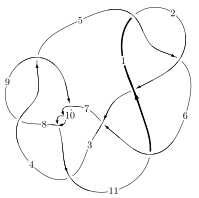
\includegraphics[width=112pt]{../../../GIT/diagram.site/Diagrams/png/332_11a_83.png}\\
\ \ \ A knot diagram\footnotemark}&
\allowdisplaybreaks
\textbf{Linearized knot diagam} \\
\cline{2-2}
 &
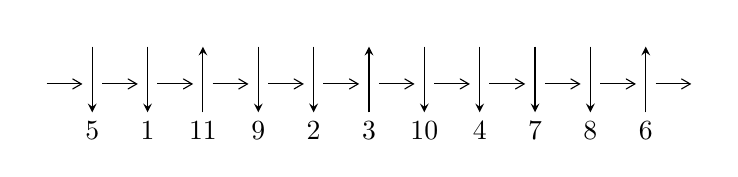
\begin{tikzpicture}[x=20pt, y=17pt]
	% nodes
	\node (C0) at (0, 0) {};
	\node (C1) at (1, 0) {};
	\node (C1U) at (1, +1) {};
	\node (C1D) at (1, -1) {5};

	\node (C2) at (2, 0) {};
	\node (C2U) at (2, +1) {};
	\node (C2D) at (2, -1) {1};

	\node (C3) at (3, 0) {};
	\node (C3U) at (3, +1) {};
	\node (C3D) at (3, -1) {11};

	\node (C4) at (4, 0) {};
	\node (C4U) at (4, +1) {};
	\node (C4D) at (4, -1) {9};

	\node (C5) at (5, 0) {};
	\node (C5U) at (5, +1) {};
	\node (C5D) at (5, -1) {2};

	\node (C6) at (6, 0) {};
	\node (C6U) at (6, +1) {};
	\node (C6D) at (6, -1) {3};

	\node (C7) at (7, 0) {};
	\node (C7U) at (7, +1) {};
	\node (C7D) at (7, -1) {10};

	\node (C8) at (8, 0) {};
	\node (C8U) at (8, +1) {};
	\node (C8D) at (8, -1) {4};

	\node (C9) at (9, 0) {};
	\node (C9U) at (9, +1) {};
	\node (C9D) at (9, -1) {7};

	\node (C10) at (10, 0) {};
	\node (C10U) at (10, +1) {};
	\node (C10D) at (10, -1) {8};

	\node (C11) at (11, 0) {};
	\node (C11U) at (11, +1) {};
	\node (C11D) at (11, -1) {6};
	\node (C12) at (12, 0) {};

	% arrows
	\draw[->,>={angle 60}]
	(C0) edge (C1) (C1) edge (C2) (C2) edge (C3) (C3) edge (C4) (C4) edge (C5) (C5) edge (C6) (C6) edge (C7) (C7) edge (C8) (C8) edge (C9) (C9) edge (C10) (C10) edge (C11) (C11) edge (C12) ;	\draw[->,>=stealth]
	(C1U) edge (C1D) (C2U) edge (C2D) (C3D) edge (C3U) (C4U) edge (C4D) (C5U) edge (C5D) (C6D) edge (C6U) (C7U) edge (C7D) (C8U) edge (C8D) (C9U) edge (C9D) (C10U) edge (C10D) (C11D) edge (C11U) ;
	\end{tikzpicture} \\
\hhline{~~} \\& 
\textbf{Solving Sequence} \\ \cline{2-2} 
 &
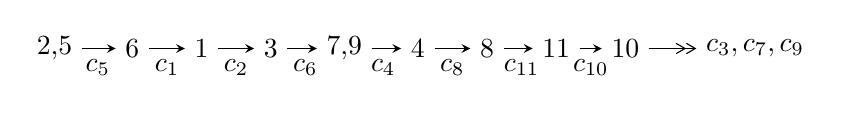
\begin{tikzpicture}[x=25pt, y=7pt]
	% node
	\node (A0) at (-1/8, 0) {2,5};
	\node (A1) at (1, 0) {6};
	\node (A2) at (2, 0) {1};
	\node (A3) at (3, 0) {3};
	\node (A4) at (65/16, 0) {7,9};
	\node (A5) at (41/8, 0) {4};
	\node (A6) at (49/8, 0) {8};
	\node (A7) at (57/8, 0) {11};
	\node (A8) at (65/8, 0) {10};
	\node (C1) at (1/2, -1) {$c_{5}$};
	\node (C2) at (3/2, -1) {$c_{1}$};
	\node (C3) at (5/2, -1) {$c_{2}$};
	\node (C4) at (7/2, -1) {$c_{6}$};
	\node (C5) at (37/8, -1) {$c_{4}$};
	\node (C6) at (45/8, -1) {$c_{8}$};
	\node (C7) at (53/8, -1) {$c_{11}$};
	\node (C8) at (61/8, -1) {$c_{10}$};
	\node (A9) at (10, 0) {$c_{3},c_{7},c_{9}$};

	% edge
	\draw[->,>=stealth]	
	(A0) edge (A1) (A1) edge (A2) (A2) edge (A3) (A3) edge (A4) (A4) edge (A5) (A5) edge (A6) (A6) edge (A7) (A7) edge (A8) ;
	\draw[->>,>={angle 60}]	
	(A8) edge (A9);
\end{tikzpicture} \\ 

\end{tabular} \\

\footnotetext{
The image of knot diagram is generated by the software ``\textbf{Draw programme}" developed by Andrew Bartholomew(\url{http://www.layer8.co.uk/maths/draw/index.htm\#Running-draw}), where we modified some parts for our purpose(\url{https://github.com/CATsTAILs/LinksPainter}).
}\phantom \\ \newline 
\centering \textbf{Ideals for irreducible components\footnotemark of $X_{\text{par}}$} 
 
\begin{align*}
I^u_{1}&=\langle 
u^{61}+2 u^{60}+\cdots+b+1,\;u^{61}+u^{60}+\cdots+a+2,\;u^{62}+2 u^{61}+\cdots+5 u+1\rangle \\
I^u_{2}&=\langle 
b,\;- u^4+u^3+u^2+a- u,\;u^6- u^5- u^4+2 u^3- u+1\rangle \\
\\
\end{align*}
\raggedright * 2 irreducible components of $\dim_{\mathbb{C}}=0$, with total 68 representations.\\
\footnotetext{All coefficients of polynomials are rational numbers. But the coefficients are sometimes approximated in decimal forms when there is not enough margin.}
\newpage
\renewcommand{\arraystretch}{1}
\centering \section*{I. $I^u_{1}= \langle u^{61}+2 u^{60}+\cdots+b+1,\;u^{61}+u^{60}+\cdots+a+2,\;u^{62}+2 u^{61}+\cdots+5 u+1 \rangle$}
\flushleft \textbf{(i) Arc colorings}\\
\begin{tabular}{m{7pt} m{180pt} m{7pt} m{180pt} }
\flushright $a_{2}=$&$\begin{pmatrix}0\\u\end{pmatrix}$ \\
\flushright $a_{5}=$&$\begin{pmatrix}1\\0\end{pmatrix}$ \\
\flushright $a_{6}=$&$\begin{pmatrix}1\\u^2\end{pmatrix}$ \\
\flushright $a_{1}=$&$\begin{pmatrix}u\\u\end{pmatrix}$ \\
\flushright $a_{3}=$&$\begin{pmatrix}- u^3\\- u^3+u\end{pmatrix}$ \\
\flushright $a_{7}=$&$\begin{pmatrix}u^8- u^6+u^4+1\\u^8-2 u^6+2 u^4\end{pmatrix}$ \\
\flushright $a_{9}=$&$\begin{pmatrix}- u^{61}- u^{60}+\cdots- u-2\\- u^{61}-2 u^{60}+\cdots-3 u-1\end{pmatrix}$ \\
\flushright $a_{4}=$&$\begin{pmatrix}u^{11}-2 u^9+2 u^7- u^3\\u^{13}-3 u^{11}+5 u^9-4 u^7+2 u^5- u^3+u\end{pmatrix}$ \\
\flushright $a_{8}=$&$\begin{pmatrix}u^{61}+u^{60}+\cdots+4 u-1\\u^{61}+2 u^{60}+\cdots+6 u+1\end{pmatrix}$ \\
\flushright $a_{11}=$&$\begin{pmatrix}u^3\\u^5- u^3+u\end{pmatrix}$ \\
\flushright $a_{10}=$&$\begin{pmatrix}- u^{59}- u^{58}+\cdots+u-1\\u^{34}-8 u^{32}+\cdots+u^2+2 u\end{pmatrix}$\\ \flushright $a_{10}=$&$\begin{pmatrix}- u^{59}- u^{58}+\cdots+u-1\\u^{34}-8 u^{32}+\cdots+u^2+2 u\end{pmatrix}$\\&\end{tabular}
\flushleft \textbf{(ii) Obstruction class $= -1$}\\~\\
\flushleft \textbf{(iii) Cusp Shapes $= -8 u^{61}-10 u^{60}+\cdots-32 u-18$}\\~\\
\newpage\renewcommand{\arraystretch}{1}
\flushleft \textbf{(iv) u-Polynomials at the component}\newline \\
\begin{tabular}{m{50pt}|m{274pt}}
Crossings & \hspace{64pt}u-Polynomials at each crossing \\
\hline $$\begin{aligned}c_{1},c_{5}\end{aligned}$$&$\begin{aligned}
&u^{62}+2 u^{61}+\cdots+5 u+1
\end{aligned}$\\
\hline $$\begin{aligned}c_{2}\end{aligned}$$&$\begin{aligned}
&u^{62}+30 u^{61}+\cdots+9 u+1
\end{aligned}$\\
\hline $$\begin{aligned}c_{3}\end{aligned}$$&$\begin{aligned}
&u^{62}+6 u^{61}+\cdots+2661 u+145
\end{aligned}$\\
\hline $$\begin{aligned}c_{4},c_{8}\end{aligned}$$&$\begin{aligned}
&u^{62}- u^{61}+\cdots-64 u-64
\end{aligned}$\\
\hline $$\begin{aligned}c_{6}\end{aligned}$$&$\begin{aligned}
&u^{62}-2 u^{61}+\cdots-55 u+25
\end{aligned}$\\
\hline $$\begin{aligned}c_{7},c_{9},c_{10}\end{aligned}$$&$\begin{aligned}
&u^{62}-7 u^{61}+\cdots+4 u-1
\end{aligned}$\\
\hline $$\begin{aligned}c_{11}\end{aligned}$$&$\begin{aligned}
&u^{62}+6 u^{61}+\cdots+15 u-53
\end{aligned}$\\
\hline
\end{tabular}\\~\\
\newpage\renewcommand{\arraystretch}{1}
\flushleft \textbf{(v) Riley Polynomials at the component}\newline \\
\begin{tabular}{m{50pt}|m{274pt}}
Crossings & \hspace{64pt}Riley Polynomials at each crossing \\
\hline $$\begin{aligned}c_{1},c_{5}\end{aligned}$$&$\begin{aligned}
&y^{62}-30 y^{61}+\cdots-9 y+1
\end{aligned}$\\
\hline $$\begin{aligned}c_{2}\end{aligned}$$&$\begin{aligned}
&y^{62}+6 y^{61}+\cdots- y+1
\end{aligned}$\\
\hline $$\begin{aligned}c_{3}\end{aligned}$$&$\begin{aligned}
&y^{62}+30 y^{61}+\cdots-4814861 y+21025
\end{aligned}$\\
\hline $$\begin{aligned}c_{4},c_{8}\end{aligned}$$&$\begin{aligned}
&y^{62}-39 y^{61}+\cdots-24576 y+4096
\end{aligned}$\\
\hline $$\begin{aligned}c_{6}\end{aligned}$$&$\begin{aligned}
&y^{62}-6 y^{61}+\cdots-21225 y+625
\end{aligned}$\\
\hline $$\begin{aligned}c_{7},c_{9},c_{10}\end{aligned}$$&$\begin{aligned}
&y^{62}-61 y^{61}+\cdots-2 y+1
\end{aligned}$\\
\hline $$\begin{aligned}c_{11}\end{aligned}$$&$\begin{aligned}
&y^{62}+18 y^{61}+\cdots-187845 y+2809
\end{aligned}$\\
\hline
\end{tabular}\\~\\
\newpage\flushleft \textbf{(vi) Complex Volumes and Cusp Shapes}
$$\begin{array}{c|c|c}  
\text{Solutions to }I^u_{1}& \I (\text{vol} + \sqrt{-1}CS) & \text{Cusp shape}\\
 \hline 
\begin{aligned}
u &= -0.679176 + 0.662219 I \\
a &= -0.18999 - 1.63576 I \\
b &= -1.295360 + 0.556741 I\end{aligned}
 & -5.37098 + 7.45017 I & -7.08441 - 6.24513 I \\ \hline\begin{aligned}
u &= -0.679176 - 0.662219 I \\
a &= -0.18999 + 1.63576 I \\
b &= -1.295360 - 0.556741 I\end{aligned}
 & -5.37098 - 7.45017 I & -7.08441 + 6.24513 I \\ \hline\begin{aligned}
u &= -1.05421\phantom{ +0.000000I} \\
a &= \phantom{-}1.10748\phantom{ +0.000000I} \\
b &= \phantom{-}1.16790\phantom{ +0.000000I}\end{aligned}
 & -6.55973\phantom{ +0.000000I} & -13.9110\phantom{ +0.000000I} \\ \hline\begin{aligned}
u &= -0.932912 + 0.505303 I \\
a &= -0.286341 - 0.182563 I \\
b &= -0.872270 - 0.423516 I\end{aligned}
 & -0.300969 + 0.586034 I & -4.56074 + 0. I\phantom{ +0.000000I} \\ \hline\begin{aligned}
u &= -0.932912 - 0.505303 I \\
a &= -0.286341 + 0.182563 I \\
b &= -0.872270 + 0.423516 I\end{aligned}
 & -0.300969 - 0.586034 I & -4.56074 + 0. I\phantom{ +0.000000I} \\ \hline\begin{aligned}
u &= -0.888402 + 0.597163 I \\
a &= -0.268028 + 0.435451 I \\
b &= \phantom{-}1.268860 + 0.490752 I\end{aligned}
 & -5.99141 - 2.56355 I & -8.39249 + 0. I\phantom{ +0.000000I} \\ \hline\begin{aligned}
u &= -0.888402 - 0.597163 I \\
a &= -0.268028 - 0.435451 I \\
b &= \phantom{-}1.268860 - 0.490752 I\end{aligned}
 & -5.99141 + 2.56355 I & -8.39249 + 0. I\phantom{ +0.000000I} \\ \hline\begin{aligned}
u &= -1.044380 + 0.283828 I \\
a &= -0.214117 + 0.472824 I \\
b &= -0.119180 + 0.531653 I\end{aligned}
 & -2.21180 + 0.64861 I & -5.56487 + 0. I\phantom{ +0.000000I} \\ \hline\begin{aligned}
u &= -1.044380 - 0.283828 I \\
a &= -0.214117 - 0.472824 I \\
b &= -0.119180 - 0.531653 I\end{aligned}
 & -2.21180 - 0.64861 I & -5.56487 + 0. I\phantom{ +0.000000I} \\ \hline\begin{aligned}
u &= \phantom{-}0.998620 + 0.452665 I \\
a &= \phantom{-}1.57838 - 1.39707 I \\
b &= \phantom{-}0.447746 + 0.704295 I\end{aligned}
 & -2.95435 - 2.01994 I & \phantom{-0.000000 } 0\\
 \hline 
 \end{array}$$\newpage$$\begin{array}{c|c|c}  
\text{Solutions to }I^u_{1}& \I (\text{vol} + \sqrt{-1}CS) & \text{Cusp shape}\\
 \hline 
\begin{aligned}
u &= \phantom{-}0.998620 - 0.452665 I \\
a &= \phantom{-}1.57838 + 1.39707 I \\
b &= \phantom{-}0.447746 - 0.704295 I\end{aligned}
 & -2.95435 + 2.01994 I & \phantom{-0.000000 } 0 \\ \hline\begin{aligned}
u &= \phantom{-}0.481047 + 0.736102 I \\
a &= \phantom{-}0.842249 - 0.094453 I \\
b &= -1.011210 + 0.071067 I\end{aligned}
 & -1.38122 + 1.31968 I & -7.80241 - 0.73411 I \\ \hline\begin{aligned}
u &= \phantom{-}0.481047 - 0.736102 I \\
a &= \phantom{-}0.842249 + 0.094453 I \\
b &= -1.011210 - 0.071067 I\end{aligned}
 & -1.38122 - 1.31968 I & -7.80241 + 0.73411 I \\ \hline\begin{aligned}
u &= -0.641660 + 0.597312 I \\
a &= \phantom{-}0.58108 + 1.47763 I \\
b &= \phantom{-}1.016340 - 0.406662 I\end{aligned}
 & \phantom{-}0.53323 + 3.83893 I & -3.44231 - 6.73024 I \\ \hline\begin{aligned}
u &= -0.641660 - 0.597312 I \\
a &= \phantom{-}0.58108 - 1.47763 I \\
b &= \phantom{-}1.016340 + 0.406662 I\end{aligned}
 & \phantom{-}0.53323 - 3.83893 I & -3.44231 + 6.73024 I \\ \hline\begin{aligned}
u &= -0.314518 + 0.789523 I \\
a &= -0.542467 + 1.246720 I \\
b &= -1.36124 - 0.62963 I\end{aligned}
 & -7.24174 - 9.68169 I & -8.05456 + 5.30748 I \\ \hline\begin{aligned}
u &= -0.314518 - 0.789523 I \\
a &= -0.542467 - 1.246720 I \\
b &= -1.36124 + 0.62963 I\end{aligned}
 & -7.24174 + 9.68169 I & -8.05456 - 5.30748 I \\ \hline\begin{aligned}
u &= -1.041180 + 0.492997 I \\
a &= \phantom{-}1.117260 + 0.139741 I \\
b &= \phantom{-}0.726241 + 0.454281 I\end{aligned}
 & -2.51432 + 4.16837 I & \phantom{-0.000000 } 0 \\ \hline\begin{aligned}
u &= -1.041180 - 0.492997 I \\
a &= \phantom{-}1.117260 - 0.139741 I \\
b &= \phantom{-}0.726241 - 0.454281 I\end{aligned}
 & -2.51432 - 4.16837 I & \phantom{-0.000000 } 0 \\ \hline\begin{aligned}
u &= \phantom{-}0.653736 + 0.523730 I \\
a &= \phantom{-}0.63997 - 1.29536 I \\
b &= -0.226464 + 0.938981 I\end{aligned}
 & -1.96315 - 1.86835 I & -5.30999 + 3.44397 I\\
 \hline 
 \end{array}$$\newpage$$\begin{array}{c|c|c}  
\text{Solutions to }I^u_{1}& \I (\text{vol} + \sqrt{-1}CS) & \text{Cusp shape}\\
 \hline 
\begin{aligned}
u &= \phantom{-}0.653736 - 0.523730 I \\
a &= \phantom{-}0.63997 + 1.29536 I \\
b &= -0.226464 - 0.938981 I\end{aligned}
 & -1.96315 + 1.86835 I & -5.30999 - 3.44397 I \\ \hline\begin{aligned}
u &= \phantom{-}1.132590 + 0.263688 I \\
a &= -2.56165 + 0.11158 I \\
b &= -1.188730 + 0.323346 I\end{aligned}
 & -5.39540 + 2.71872 I & \phantom{-0.000000 } 0 \\ \hline\begin{aligned}
u &= \phantom{-}1.132590 - 0.263688 I \\
a &= -2.56165 - 0.11158 I \\
b &= -1.188730 - 0.323346 I\end{aligned}
 & -5.39540 - 2.71872 I & \phantom{-0.000000 } 0 \\ \hline\begin{aligned}
u &= \phantom{-}1.030730 + 0.541655 I \\
a &= -0.821984 + 0.953842 I \\
b &= -0.534592 - 0.594863 I\end{aligned}
 & \phantom{-}0.73820 - 4.68678 I & \phantom{-0.000000 } 0 \\ \hline\begin{aligned}
u &= \phantom{-}1.030730 - 0.541655 I \\
a &= -0.821984 - 0.953842 I \\
b &= -0.534592 + 0.594863 I\end{aligned}
 & \phantom{-}0.73820 + 4.68678 I & \phantom{-0.000000 } 0 \\ \hline\begin{aligned}
u &= \phantom{-}1.127010 + 0.311355 I \\
a &= \phantom{-}2.80083 - 0.32064 I \\
b &= \phantom{-}1.166360 + 0.082032 I\end{aligned}
 & -5.92111 - 2.41747 I & \phantom{-0.000000 } 0 \\ \hline\begin{aligned}
u &= \phantom{-}1.127010 - 0.311355 I \\
a &= \phantom{-}2.80083 + 0.32064 I \\
b &= \phantom{-}1.166360 - 0.082032 I\end{aligned}
 & -5.92111 + 2.41747 I & \phantom{-0.000000 } 0 \\ \hline\begin{aligned}
u &= -1.134480 + 0.286998 I \\
a &= \phantom{-}0.391333 - 1.078140 I \\
b &= \phantom{-}0.127006 - 1.226480 I\end{aligned}
 & -7.77591 - 0.20988 I & \phantom{-0.000000 } 0 \\ \hline\begin{aligned}
u &= -1.134480 - 0.286998 I \\
a &= \phantom{-}0.391333 + 1.078140 I \\
b &= \phantom{-}0.127006 + 1.226480 I\end{aligned}
 & -7.77591 + 0.20988 I & \phantom{-0.000000 } 0 \\ \hline\begin{aligned}
u &= \phantom{-}1.163140 + 0.238954 I \\
a &= \phantom{-}2.30064 - 0.28329 I \\
b &= \phantom{-}1.40475 - 0.59693 I\end{aligned}
 & -11.90540 + 6.70531 I & \phantom{-0.000000 } 0\\
 \hline 
 \end{array}$$\newpage$$\begin{array}{c|c|c}  
\text{Solutions to }I^u_{1}& \I (\text{vol} + \sqrt{-1}CS) & \text{Cusp shape}\\
 \hline 
\begin{aligned}
u &= \phantom{-}1.163140 - 0.238954 I \\
a &= \phantom{-}2.30064 + 0.28329 I \\
b &= \phantom{-}1.40475 + 0.59693 I\end{aligned}
 & -11.90540 - 6.70531 I & \phantom{-0.000000 } 0 \\ \hline\begin{aligned}
u &= -0.308882 + 0.748072 I \\
a &= \phantom{-}0.91507 - 1.12308 I \\
b &= \phantom{-}1.161680 + 0.400372 I\end{aligned}
 & -1.02712 - 5.59716 I & -5.41314 + 5.44677 I \\ \hline\begin{aligned}
u &= -0.308882 - 0.748072 I \\
a &= \phantom{-}0.91507 + 1.12308 I \\
b &= \phantom{-}1.161680 - 0.400372 I\end{aligned}
 & -1.02712 + 5.59716 I & -5.41314 - 5.44677 I \\ \hline\begin{aligned}
u &= \phantom{-}0.500918 + 0.616350 I \\
a &= -0.430610 + 0.666088 I \\
b &= \phantom{-}0.428614 - 0.571553 I\end{aligned}
 & \phantom{-}2.29604 + 0.10479 I & \phantom{-}1.82899 - 0.07874 I \\ \hline\begin{aligned}
u &= \phantom{-}0.500918 - 0.616350 I \\
a &= -0.430610 - 0.666088 I \\
b &= \phantom{-}0.428614 + 0.571553 I\end{aligned}
 & \phantom{-}2.29604 - 0.10479 I & \phantom{-}1.82899 + 0.07874 I \\ \hline\begin{aligned}
u &= \phantom{-}1.057630 + 0.597978 I \\
a &= \phantom{-}0.024817 - 1.263810 I \\
b &= \phantom{-}1.004900 + 0.137217 I\end{aligned}
 & -3.08504 - 6.39994 I & \phantom{-0.000000 } 0 \\ \hline\begin{aligned}
u &= \phantom{-}1.057630 - 0.597978 I \\
a &= \phantom{-}0.024817 + 1.263810 I \\
b &= \phantom{-}1.004900 - 0.137217 I\end{aligned}
 & -3.08504 + 6.39994 I & \phantom{-0.000000 } 0 \\ \hline\begin{aligned}
u &= \phantom{-}1.164990 + 0.345279 I \\
a &= -2.73197 + 0.41008 I \\
b &= -1.47526 - 0.42876 I\end{aligned}
 & -13.1853 - 5.6875 I & \phantom{-0.000000 } 0 \\ \hline\begin{aligned}
u &= \phantom{-}1.164990 - 0.345279 I \\
a &= -2.73197 - 0.41008 I \\
b &= -1.47526 + 0.42876 I\end{aligned}
 & -13.1853 + 5.6875 I & \phantom{-0.000000 } 0 \\ \hline\begin{aligned}
u &= \phantom{-}0.284471 + 0.730649 I \\
a &= \phantom{-}0.544524 + 0.656664 I \\
b &= -0.217691 - 1.178550 I\end{aligned}
 & -3.57456 + 3.20100 I & -7.28225 - 2.52053 I\\
 \hline 
 \end{array}$$\newpage$$\begin{array}{c|c|c}  
\text{Solutions to }I^u_{1}& \I (\text{vol} + \sqrt{-1}CS) & \text{Cusp shape}\\
 \hline 
\begin{aligned}
u &= \phantom{-}0.284471 - 0.730649 I \\
a &= \phantom{-}0.544524 - 0.656664 I \\
b &= -0.217691 + 1.178550 I\end{aligned}
 & -3.57456 - 3.20100 I & -7.28225 + 2.52053 I \\ \hline\begin{aligned}
u &= \phantom{-}0.373838 + 0.680597 I \\
a &= -0.383069 - 0.431263 I \\
b &= \phantom{-}0.252931 + 0.605320 I\end{aligned}
 & \phantom{-}1.74078 + 1.61529 I & \phantom{-}1.05360 - 1.69724 I \\ \hline\begin{aligned}
u &= \phantom{-}0.373838 - 0.680597 I \\
a &= -0.383069 + 0.431263 I \\
b &= \phantom{-}0.252931 - 0.605320 I\end{aligned}
 & \phantom{-}1.74078 - 1.61529 I & \phantom{-}1.05360 + 1.69724 I \\ \hline\begin{aligned}
u &= \phantom{-}1.093600 + 0.552610 I \\
a &= \phantom{-}0.849609 + 0.340920 I \\
b &= -0.203226 + 0.645415 I\end{aligned}
 & -0.35142 - 6.38903 I & \phantom{-0.000000 } 0 \\ \hline\begin{aligned}
u &= \phantom{-}1.093600 - 0.552610 I \\
a &= \phantom{-}0.849609 - 0.340920 I \\
b &= -0.203226 - 0.645415 I\end{aligned}
 & -0.35142 + 6.38903 I & \phantom{-0.000000 } 0 \\ \hline\begin{aligned}
u &= -0.164713 + 0.739758 I \\
a &= \phantom{-}0.592183 - 0.152334 I \\
b &= \phantom{-}1.43644 - 0.36265 I\end{aligned}
 & -9.25615 + 2.11576 I & -10.25958 - 1.04111 I \\ \hline\begin{aligned}
u &= -0.164713 - 0.739758 I \\
a &= \phantom{-}0.592183 + 0.152334 I \\
b &= \phantom{-}1.43644 + 0.36265 I\end{aligned}
 & -9.25615 - 2.11576 I & -10.25958 + 1.04111 I \\ \hline\begin{aligned}
u &= -1.124020 + 0.532845 I \\
a &= \phantom{-}2.12343 + 1.58416 I \\
b &= \phantom{-}1.160650 - 0.052166 I\end{aligned}
 & -4.41765 + 5.31598 I & \phantom{-0.000000 } 0 \\ \hline\begin{aligned}
u &= -1.124020 - 0.532845 I \\
a &= \phantom{-}2.12343 - 1.58416 I \\
b &= \phantom{-}1.160650 + 0.052166 I\end{aligned}
 & -4.41765 - 5.31598 I & \phantom{-0.000000 } 0 \\ \hline\begin{aligned}
u &= \phantom{-}1.130270 + 0.545573 I \\
a &= -1.47482 - 0.61853 I \\
b &= \phantom{-}0.240687 - 1.232260 I\end{aligned}
 & -6.02650 - 8.03942 I & \phantom{-0.000000 } 0\\
 \hline 
 \end{array}$$\newpage$$\begin{array}{c|c|c}  
\text{Solutions to }I^u_{1}& \I (\text{vol} + \sqrt{-1}CS) & \text{Cusp shape}\\
 \hline 
\begin{aligned}
u &= \phantom{-}1.130270 - 0.545573 I \\
a &= -1.47482 + 0.61853 I \\
b &= \phantom{-}0.240687 + 1.232260 I\end{aligned}
 & -6.02650 + 8.03942 I & \phantom{-0.000000 } 0 \\ \hline\begin{aligned}
u &= -1.152310 + 0.504519 I \\
a &= -1.60293 - 1.74806 I \\
b &= -1.49016 - 0.33112 I\end{aligned}
 & -12.10490 + 2.50349 I & \phantom{-0.000000 } 0 \\ \hline\begin{aligned}
u &= -1.152310 - 0.504519 I \\
a &= -1.60293 + 1.74806 I \\
b &= -1.49016 + 0.33112 I\end{aligned}
 & -12.10490 - 2.50349 I & \phantom{-0.000000 } 0 \\ \hline\begin{aligned}
u &= -1.129340 + 0.556780 I \\
a &= -2.25146 - 1.88634 I \\
b &= -1.201730 + 0.414457 I\end{aligned}
 & -3.42397 + 10.52990 I & \phantom{-0.000000 } 0 \\ \hline\begin{aligned}
u &= -1.129340 - 0.556780 I \\
a &= -2.25146 + 1.88634 I \\
b &= -1.201730 - 0.414457 I\end{aligned}
 & -3.42397 - 10.52990 I & \phantom{-0.000000 } 0 \\ \hline\begin{aligned}
u &= -0.263424 + 0.692134 I \\
a &= -1.158110 + 0.521094 I \\
b &= -1.087530 - 0.017394 I\end{aligned}
 & -1.96243 - 0.62500 I & -7.94260 - 0.21317 I \\ \hline\begin{aligned}
u &= -0.263424 - 0.692134 I \\
a &= -1.158110 - 0.521094 I \\
b &= -1.087530 + 0.017394 I\end{aligned}
 & -1.96243 + 0.62500 I & -7.94260 + 0.21317 I \\ \hline\begin{aligned}
u &= -1.140580 + 0.570161 I \\
a &= \phantom{-}2.21593 + 2.00462 I \\
b &= \phantom{-}1.37560 - 0.65487 I\end{aligned}
 & -9.6807 + 14.7703 I & \phantom{-0.000000 } 0 \\ \hline\begin{aligned}
u &= -1.140580 - 0.570161 I \\
a &= \phantom{-}2.21593 - 2.00462 I \\
b &= \phantom{-}1.37560 + 0.65487 I\end{aligned}
 & -9.6807 - 14.7703 I & \phantom{-0.000000 } 0 \\ \hline\begin{aligned}
u &= -0.481620 + 0.441597 I \\
a &= -1.41313 - 0.85379 I \\
b &= -0.708754 + 0.202332 I\end{aligned}
 & -0.830855 - 0.117361 I & -8.01128 - 1.52685 I\\
 \hline 
 \end{array}$$\newpage$$\begin{array}{c|c|c}  
\text{Solutions to }I^u_{1}& \I (\text{vol} + \sqrt{-1}CS) & \text{Cusp shape}\\
 \hline 
\begin{aligned}
u &= -0.481620 - 0.441597 I \\
a &= -1.41313 + 0.85379 I \\
b &= -0.708754 - 0.202332 I\end{aligned}
 & -0.830855 + 0.117361 I & -8.01128 + 1.52685 I \\ \hline\begin{aligned}
u &= -0.447785\phantom{ +0.000000I} \\
a &= -1.48076\phantom{ +0.000000I} \\
b &= -0.618691\phantom{ +0.000000I}\end{aligned}
 & -0.957809\phantom{ +0.000000I} & -9.90970\phantom{ +0.000000I}\\
 \hline 
 \end{array}$$\newpage\newpage\renewcommand{\arraystretch}{1}
\centering \section*{II. $I^u_{2}= \langle b,\;- u^4+u^3+u^2+a- u,\;u^6- u^5- u^4+2 u^3- u+1 \rangle$}
\flushleft \textbf{(i) Arc colorings}\\
\begin{tabular}{m{7pt} m{180pt} m{7pt} m{180pt} }
\flushright $a_{2}=$&$\begin{pmatrix}0\\u\end{pmatrix}$ \\
\flushright $a_{5}=$&$\begin{pmatrix}1\\0\end{pmatrix}$ \\
\flushright $a_{6}=$&$\begin{pmatrix}1\\u^2\end{pmatrix}$ \\
\flushright $a_{1}=$&$\begin{pmatrix}u\\u\end{pmatrix}$ \\
\flushright $a_{3}=$&$\begin{pmatrix}- u^3\\- u^3+u\end{pmatrix}$ \\
\flushright $a_{7}=$&$\begin{pmatrix}- u^3\\- u^5+u^3- u\end{pmatrix}$ \\
\flushright $a_{9}=$&$\begin{pmatrix}u^4- u^3- u^2+u\\0\end{pmatrix}$ \\
\flushright $a_{4}=$&$\begin{pmatrix}1\\0\end{pmatrix}$ \\
\flushright $a_{8}=$&$\begin{pmatrix}u^4- u^3- u^2+u\\0\end{pmatrix}$ \\
\flushright $a_{11}=$&$\begin{pmatrix}u^3\\u^5- u^3+u\end{pmatrix}$ \\
\flushright $a_{10}=$&$\begin{pmatrix}u^4- u^2+u\\u^5- u^3+u\end{pmatrix}$\\ \flushright $a_{10}=$&$\begin{pmatrix}u^4- u^2+u\\u^5- u^3+u\end{pmatrix}$\\&\end{tabular}
\flushleft \textbf{(ii) Obstruction class $= 1$}\\~\\
\flushleft \textbf{(iii) Cusp Shapes $= 4 u^4-5 u^2+5 u-5$}\\~\\
\newpage\renewcommand{\arraystretch}{1}
\flushleft \textbf{(iv) u-Polynomials at the component}\newline \\
\begin{tabular}{m{50pt}|m{274pt}}
Crossings & \hspace{64pt}u-Polynomials at each crossing \\
\hline $$\begin{aligned}c_{1},c_{3},c_{6}\end{aligned}$$&$\begin{aligned}
&u^6+u^5- u^4-2 u^3+u+1
\end{aligned}$\\
\hline $$\begin{aligned}c_{2},c_{11}\end{aligned}$$&$\begin{aligned}
&u^6+3 u^5+5 u^4+4 u^3+2 u^2+u+1
\end{aligned}$\\
\hline $$\begin{aligned}c_{4},c_{8}\end{aligned}$$&$\begin{aligned}
&u^6
\end{aligned}$\\
\hline $$\begin{aligned}c_{5}\end{aligned}$$&$\begin{aligned}
&u^6- u^5- u^4+2 u^3- u+1
\end{aligned}$\\
\hline $$\begin{aligned}c_{7}\end{aligned}$$&$\begin{aligned}
&(u-1)^6
\end{aligned}$\\
\hline $$\begin{aligned}c_{9},c_{10}\end{aligned}$$&$\begin{aligned}
&(u+1)^6
\end{aligned}$\\
\hline
\end{tabular}\\~\\
\newpage\renewcommand{\arraystretch}{1}
\flushleft \textbf{(v) Riley Polynomials at the component}\newline \\
\begin{tabular}{m{50pt}|m{274pt}}
Crossings & \hspace{64pt}Riley Polynomials at each crossing \\
\hline $$\begin{aligned}c_{1},c_{3},c_{5}\\c_{6}\end{aligned}$$&$\begin{aligned}
&y^6-3 y^5+5 y^4-4 y^3+2 y^2- y+1
\end{aligned}$\\
\hline $$\begin{aligned}c_{2},c_{11}\end{aligned}$$&$\begin{aligned}
&y^6+y^5+5 y^4+6 y^2+3 y+1
\end{aligned}$\\
\hline $$\begin{aligned}c_{4},c_{8}\end{aligned}$$&$\begin{aligned}
&y^6
\end{aligned}$\\
\hline $$\begin{aligned}c_{7},c_{9},c_{10}\end{aligned}$$&$\begin{aligned}
&(y-1)^6
\end{aligned}$\\
\hline
\end{tabular}\\~\\
\newpage\flushleft \textbf{(vi) Complex Volumes and Cusp Shapes}
$$\begin{array}{c|c|c}  
\text{Solutions to }I^u_{2}& \I (\text{vol} + \sqrt{-1}CS) & \text{Cusp shape}\\
 \hline 
\begin{aligned}
u &= -1.002190 + 0.295542 I \\
a &= -0.685196 - 1.063260 I \\
b &= \phantom{-0.000000 } 0\end{aligned}
 & -3.53554 + 0.92430 I & -12.63596 + 0.09369 I \\ \hline\begin{aligned}
u &= -1.002190 - 0.295542 I \\
a &= -0.685196 + 1.063260 I \\
b &= \phantom{-0.000000 } 0\end{aligned}
 & -3.53554 - 0.92430 I & -12.63596 - 0.09369 I \\ \hline\begin{aligned}
u &= \phantom{-}0.428243 + 0.664531 I \\
a &= \phantom{-}0.917982 - 0.270708 I \\
b &= \phantom{-0.000000 } 0\end{aligned}
 & \phantom{-}0.245672 + 0.924305 I & -2.59683 - 0.69886 I \\ \hline\begin{aligned}
u &= \phantom{-}0.428243 - 0.664531 I \\
a &= \phantom{-}0.917982 + 0.270708 I \\
b &= \phantom{-0.000000 } 0\end{aligned}
 & \phantom{-}0.245672 - 0.924305 I & -2.59683 + 0.69886 I \\ \hline\begin{aligned}
u &= \phantom{-}1.073950 + 0.558752 I \\
a &= -0.732786 - 0.381252 I \\
b &= \phantom{-0.000000 } 0\end{aligned}
 & -1.64493 - 5.69302 I & -6.76721 + 4.86918 I \\ \hline\begin{aligned}
u &= \phantom{-}1.073950 - 0.558752 I \\
a &= -0.732786 + 0.381252 I \\
b &= \phantom{-0.000000 } 0\end{aligned}
 & -1.64493 + 5.69302 I & -6.76721 - 4.86918 I\\
 \hline 
 \end{array}$$\newpage
\newpage\renewcommand{\arraystretch}{1}
\centering \section*{ III. u-Polynomials}
\begin{tabular}{m{50pt}|m{274pt}}
Crossings & \hspace{64pt}u-Polynomials at each crossing \\
\hline $$\begin{aligned}c_{1}\end{aligned}$$&$\begin{aligned}
&(u^6+u^5- u^4-2 u^3+u+1)(u^{62}+2 u^{61}+\cdots+5 u+1)
\end{aligned}$\\
\hline $$\begin{aligned}c_{2}\end{aligned}$$&$\begin{aligned}
&(u^6+3 u^5+5 u^4+4 u^3+2 u^2+u+1)(u^{62}+30 u^{61}+\cdots+9 u+1)
\end{aligned}$\\
\hline $$\begin{aligned}c_{3}\end{aligned}$$&$\begin{aligned}
&(u^6+u^5- u^4-2 u^3+u+1)(u^{62}+6 u^{61}+\cdots+2661 u+145)
\end{aligned}$\\
\hline $$\begin{aligned}c_{4},c_{8}\end{aligned}$$&$\begin{aligned}
&u^6(u^{62}- u^{61}+\cdots-64 u-64)
\end{aligned}$\\
\hline $$\begin{aligned}c_{5}\end{aligned}$$&$\begin{aligned}
&(u^6- u^5- u^4+2 u^3- u+1)(u^{62}+2 u^{61}+\cdots+5 u+1)
\end{aligned}$\\
\hline $$\begin{aligned}c_{6}\end{aligned}$$&$\begin{aligned}
&(u^6+u^5- u^4-2 u^3+u+1)(u^{62}-2 u^{61}+\cdots-55 u+25)
\end{aligned}$\\
\hline $$\begin{aligned}c_{7}\end{aligned}$$&$\begin{aligned}
&((u-1)^6)(u^{62}-7 u^{61}+\cdots+4 u-1)
\end{aligned}$\\
\hline $$\begin{aligned}c_{9},c_{10}\end{aligned}$$&$\begin{aligned}
&((u+1)^6)(u^{62}-7 u^{61}+\cdots+4 u-1)
\end{aligned}$\\
\hline $$\begin{aligned}c_{11}\end{aligned}$$&$\begin{aligned}
&(u^6+3 u^5+5 u^4+4 u^3+2 u^2+u+1)(u^{62}+6 u^{61}+\cdots+15 u-53)
\end{aligned}$\\
\hline
\end{tabular}\newpage\renewcommand{\arraystretch}{1}
\centering \section*{ IV. Riley Polynomials}
\begin{tabular}{m{50pt}|m{274pt}}
Crossings & \hspace{64pt}Riley Polynomials at each crossing \\
\hline $$\begin{aligned}c_{1},c_{5}\end{aligned}$$&$\begin{aligned}
&(y^6-3 y^5+5 y^4-4 y^3+2 y^2- y+1)(y^{62}-30 y^{61}+\cdots-9 y+1)
\end{aligned}$\\
\hline $$\begin{aligned}c_{2}\end{aligned}$$&$\begin{aligned}
&(y^6+y^5+5 y^4+6 y^2+3 y+1)(y^{62}+6 y^{61}+\cdots- y+1)
\end{aligned}$\\
\hline $$\begin{aligned}c_{3}\end{aligned}$$&$\begin{aligned}
&(y^6-3 y^5+5 y^4-4 y^3+2 y^2- y+1)\\
&\cdot(y^{62}+30 y^{61}+\cdots-4814861 y+21025)
\end{aligned}$\\
\hline $$\begin{aligned}c_{4},c_{8}\end{aligned}$$&$\begin{aligned}
&y^6(y^{62}-39 y^{61}+\cdots-24576 y+4096)
\end{aligned}$\\
\hline $$\begin{aligned}c_{6}\end{aligned}$$&$\begin{aligned}
&(y^6-3 y^5+5 y^4-4 y^3+2 y^2- y+1)(y^{62}-6 y^{61}+\cdots-21225 y+625)
\end{aligned}$\\
\hline $$\begin{aligned}c_{7},c_{9},c_{10}\end{aligned}$$&$\begin{aligned}
&((y-1)^6)(y^{62}-61 y^{61}+\cdots-2 y+1)
\end{aligned}$\\
\hline $$\begin{aligned}c_{11}\end{aligned}$$&$\begin{aligned}
&(y^6+y^5+5 y^4+6 y^2+3 y+1)(y^{62}+18 y^{61}+\cdots-187845 y+2809)
\end{aligned}$\\
\hline
\end{tabular}
\vskip 2pc
\end{document}